\documentclass[a4paper,10pt]{scrartcl}
\usepackage[margin=2cm,bindingoffset=0cm]{geometry}
\usepackage{ucs}
\usepackage[utf8x]{inputenc}
\usepackage[ngerman]{babel}
\usepackage{fontenc}
%\usepackage[pdftex]{graphicx}
\usepackage{listings}
\usepackage{amssymb}
\usepackage{amsmath}
\usepackage{wasysym}
\usepackage{graphicx}
\usepackage[pdftex]{hyperref}
\author{Verena Käfer (2551188), Niklas Schnelle (2573250), Peter Vollmer (2553704)}
\date{erstellt am 25.10.2010\\
Version: 1.0}
\title{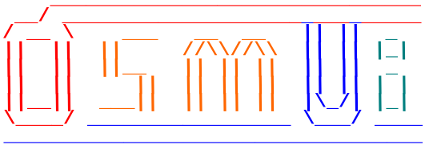
\includegraphics[width=15cm]{Logo_Osmui.png} \\ 
Spezifikation von OsmUi}

\begin{document}
\maketitle
\newpage
\tableofcontents
\newpage


\section{Einleitung}
\subsection{Zeck der Spezifikation}
\subsection{Leserkreis}
\subsection{Projektüberblick}
\subsection{Konventionen}

\section{Nichtfunktionale Anforderungen}
\subsection{Mengengerüst}
\subsection{Entwurfseinschränkungen}
\subsubsection{Systemumgebung}
\subsubsection{Layout und Gestaltung}
\subsection{Robustheit}
\subsection{Portabilität}
\subsection{Erweiterbarkeit}
\subsection{Distributionsform und Installation}

\section{Akteure}
\subsection{Benutzer}
\subsection{Testverwalter}
\subsection{Tester}
\subsection{Testauswerter}

\section{Testprotokoll-Export als PDF}
\subsection{Kopf- und Fußzeile}
\subsection{Testprotokolleigenschaften und Zusammenfassung}

\section{Benutzeroberfläche}
\subsection{Prgrammstart}
\subsection{Titelleiste des Hauptfensters}
\subsection{Startbildschirm}
\subsection{Moduswahlbildschirm}
\subsection{Allgemeine Beschreibung des Hauptfensters}
\subsubsection{Die Modusleiste}
\subsubsection{Verhalten bei Änderung der Fenstergröße}
\subsubsection{Verhalten von Rückgängig und wiederholen}
\subsubsection{Verhalten beim Erstellen von Kopien}
\subsubsection{Verhalten beim Entfernen von Elementen}
\subsubsection{Filterung der Auswahl beim Duplizieren, Kopieren und Verschieben}
\subsection{Menübefehle}
\subsubsection{Alle Testsequenzen exportieren}
\subsubsection{Ausschneiden}
\subsubsection{Ausgewählte Testsequenz exportieren}
\subsubsection{Auswertung}
\subsubsection{Beenden}
\subsubsection{Benutzerverwaltung}
\subsubsection{Durchführung}
\subsubsection{Einfügen}
\subsubsection{Einstellungen}
\subsubsection{\textit{Elememt} an das Ende verschieben}
\subsubsection{\textit{Element} an den Anfang verschieben}
\subsubsection{\textit{Element} eine Position nach ob}
\subsubsection{\textit{Element} eine Position nach unten}
\subsubsection{\textit{Element} duplizieren}
\subsubsection{\textit{Element} entfernen}
\subsubsection{Hilfe}
\subsubsection{Kopieren}
\subsubsection{Neue Testsequenz}
\subsubsection{Neuer Testfall}
\subsubsection{Neues Projekt}
\subsubsection{Programmfehler melden}
\subsubsection{Projekt öffnen}
\subsubsection{Projekt schließen}
\subsubsection{Projekt speichern}
\subsubsection{Projekt speichern unter}
\subsubsection{Rückgängig}
\subsubsection{Suchen}
\subsubsection{Test abbrechen}
\subsubsection{Test durchführen}
\subsubsection{Testdaten importieren}
\subsubsection{Testprotokoll als PDF speichern}
\subsubsection{Über}
\subsubsection{Update Prüfung}
\subsubsection{Verwaltung}
\subsubsection{Wiederholen}
\subsubsection{Zuletzt geöffnete Projekte}
\subsection{Gliederung der Menüleiste}
\subsection{Hauptfenster im Verwaltungsmodus}
\subsubsection{Der Baum}
\subsubsection{Inhaltsbereich mit Mehrfachausahl oder ohne Auswahl im Baum}
\subsubsection{Inhaltsbereich bei Auswahl einer Testsequenz}
\subsubsection{Inhaltsbereich bei Auswahl eines Testfalls}
\subsubsection{Verhalten der Eingabefelder im Inhaltsbereich}
\subsection{Hauptfenster im Durchführungsmodus}
\subsubsection{•}


\end{document}

